\chapter{Конструкторский раздел}
\label{cha:design}
В данном разделе будут рассмотрены схемы алгоритмов сортировки, введена модель вычисления трудоёмкости и в соответствии с ней подсчитана суммарная трудоёмкость для каждого из 3-х алгоритмов.
\section{Схемы алгоритмов}
\label{sec:schemes}
На рисунках 2.1-2.3 представлены схемы алгоритмов сортировки пузырьком с флагом, выбором и пирамидальной сортировки.
\begin{figure}[H]
	\centering
	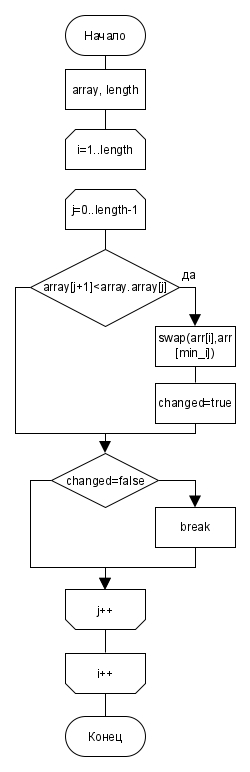
\includegraphics[height=0.8\textheight]{src/bubbleSort}
	\caption{Алгоритм сортировки пузырьком с флагом}
	\label{fig:bubblesort}
\end{figure}

\begin{figure}[H]
	\centering
	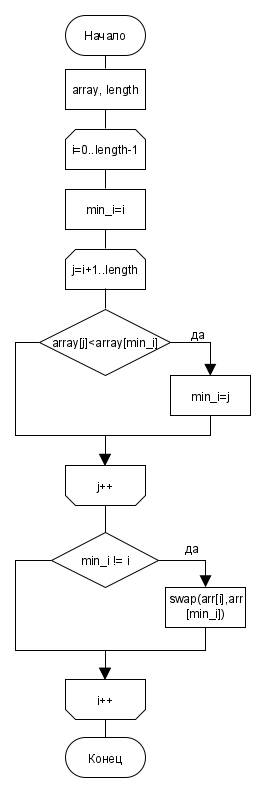
\includegraphics[height=0.8\textheight]{src/selectionSort}
	\caption{Алгоритм сортировки выбором}
	\label{fig:selectionnsort}
\end{figure}
\begin{figure}[H]
	\centering
	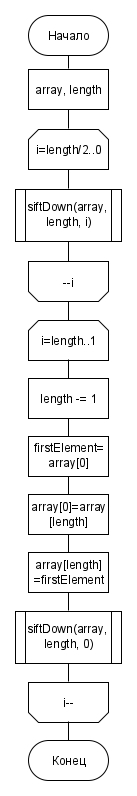
\includegraphics[height=0.8\textheight]{src/heapSort}
	\caption{Алгоритм пирамидальной сортировки}
	\label{fig:heapsort}
\end{figure}
На рисунке 2.4 представлена схема алгоритма просеивания вниз.
\begin{figure}
	\centering
	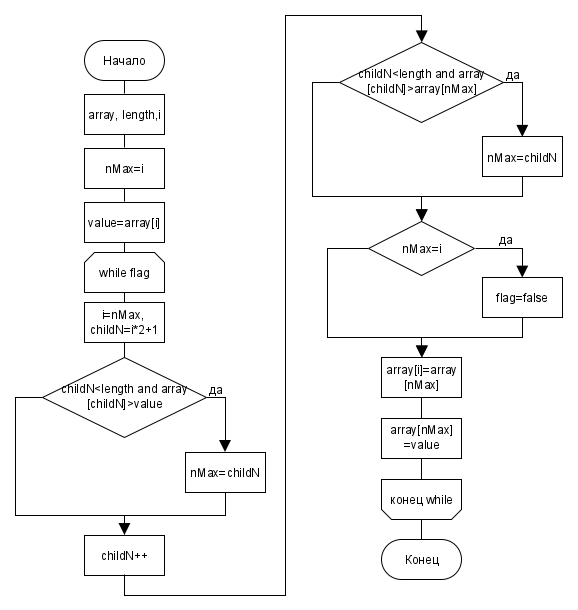
\includegraphics[height=0.7\textheight]{src/siftDown}
	\caption{Алгоритм просеивания вниз}
	\label{fig:siftdown}
\end{figure}

\section{Трудоёмкость алгоритмов}
\label{sec:labour}
Введём модель вычислений трудоёмкости:
\begin{enumerate}
	\item[1)] стоимость базовых операций 1: =,+,-,*,==,!=,<,>,<=,>=,>>,+=,-=,*=,/=,[],<<,>>;
	\item[2)] оценка трудоёмкости цикла $f_{for}=f_{init}+f_{comp}+N(f_{body}+f_{inc}+f_{comp})$;
	\item[3)] оценка трудоёмкости условного оператора, стоимость перехода положим 0, тогда
	\begin{equation}
f_{if}=f_{condition}+\begin{cases}
min(f_{1},f_{2})-\text{лучший случай}\\
max(f_{1},f_{2})-\text{худший случай}\\
\end{cases}
	\end{equation} 
\end{enumerate}
\subsection{Сортировка пузырьком с флагом}
\label{subsec:bubble}
\textbf{Лучший случай:} массив, отсортированный в правильном порядке, в данном случае вложенный цикл выполниться всего 1 раз, после чего функция завершится $f=3+3+(n-1)(3+3)+1=6n+1$.

\textbf{Худший случай:} массив, отсортированный в обратном порядке, что вызовет необходимость каждый раз производить обмен.
\begin{equation}
\begin{split}
&f=3+(n-1)(3+3)+\frac{1+(n-1)}{2}(n-1)(3+3+5+3+1)=\\
&=3+6n-6+\frac{n-1+n^2-2n+1}{2}*15=7.5n^2-1.5n-3
\end{split}
\end{equation}
\subsection{Сортировка вставками}
\label{subsec:insertion}
\textbf{Лучший случай:} отсортированный массив, при этом всё равно будут проверяться все элементы массива, но не будет выполнено ни одного обмена. Трудоёмкость составит:
\begin{equation}
\begin{split}
&f=3+(n-1)*(1+2+1+2+1+(\frac{1+n}{2})(2+3)+1)=\\
&=3+(n-1)*(8+2.5n+2.5)=2.5n^2+7.5n-7.5
\end{split}
\end{equation}

\textbf{Худший случай:} массив отсортирован в обратном порядке, в связи с чем на каждом шаге внутреннего цикла будет происходить переприсваивание, и будет происходить обмен:
\begin{equation}
\begin{split}
&f=3+(n-1)*(1+2+1+2+1+(\frac{1+n}{2})(2+3+1)+1+7)=\\
&=3+(n-1)*(15+3n+3)=3n^2+15n-15
\end{split}
\end{equation}
\subsection{Пирамидальная сортировка}
\label{subsec:heap}
Трудоёмкость алгоритма сортировки с учётом построения пирамиды будет равно $f=O(n\ln n)$ для лучшего, худшего и среднего случаев.


\section{Выводы}
\label{sec:design_conclusion}
В данном разделе были рассмотрены схемы алгоритмов сортировки, введена модель вычисления трудоёмкости, рассчитаны трудоёмкости алгоритмов. Из формул видно, что наиболее эффективный в общем случае -- алгоритм пирамидальной сортировки, в то время как сортировка пузырьком с флагом наименее трудоёмкая при наилучшем случае.
